\graphicspath{{./designDocImages/}}

\section{Introduction}

In order to investigate the research question, the development of a game was needed. A number of limitations were placed on the game, however. To begin with, the game had to be able to incorporate both gestures and direct manipulation in a way that did not adversely effect the playability of either version. It also had to present the opportunity for creating an interface that used elements of both. Another important consideration was that the game itself had to be of a relatively limited scope given the time constraints for development. However, despite this, the game should still be sufficiently involving so as to create a flow state within the player. This is necessary as the goal of much of the experimentation is to measure this flow state for each interface type. The following sections describe the design and implementation of a three-dimensional puzzle game where players attempt to match blocks of the same colour in order to score points.


\section{Game design of \emph{Hexahedron}}

\subsection{Brief overview}
Players will arrange different coloured blocks, which are initially grouped in a three-dimensional \gls{shape}, so that blocks of the same colour are next to each other. These blocks can then be removed, with the number of blocks removed at a time being exponentially related to one's score. Three different interface versions of \emph{Hexahedron} will be implemented in order to test the hypothesis under study. These include a gestural, direct manipulation and mixed interface. The gestural interface will use touch-based gestures in order to control block manipulations, while the direct manipulation version will employ buttons. The mixed interface will use a combination of the previous two. A mixed interface was added so that one can determine whether gestures or direct manipulation are appropriate for some controls, but not for all. \emph{Hexahedron} will be specifically implemented for the Apple iPad.

\subsection{Style and genre}
\emph{Hexahedron} aims to expand upon existing matching-style puzzle games by introducing a third dimension. That is, while it will bear some similarity to games such as \emph{Same} and \emph{Bejewelled}, it will expand on the basic premise of these games by allowing players to also arrange elements in the third dimension. The game will consist of a three-dimensional block made up of a number of small coloured cubes. Each cube will be consistently coloured, that is, all of its faces will share the same colour. This third dimension creates an additional element within game-play, as cubes can now be grouped together in more than just two dimensions. This allows for a more challenging experience that will encourage and help develop the spatial thinking skills of its players. The touch nature of the interface also allows for controls to be implemented through the use of gestures, which will hopefully increase flow and the ease with which the game can be played. In addition, it may give players the feeling that they are physically manipulating the three-dimensional object.


\subsection{Core game-play}
The aim of \emph{Hexahedron} is to remove as many blocks in as large a \gls{grouped} as possible. As the score received is related to the number of blocks removed, players should attempt to remove as many blocks at one time as possible. Players are able to rearrange blocks by using the predefined movement techniques discussed below. The aim of the game is to get as high a score as possible. The previous best score will be displayed underneath the current game's score.


\subsubsection{Scoring system}
When removing blocks from the screen, scores will be determined as follows, where \emph{S} is the final score and \emph{n} is the number of blocks removed:
\[  S = S + 2 \times n \]

\subsection{View controls}
\subsubsection{Rotation}
Rotation controls will be implemented so that the \gls{shape} can be rotated in one of the four cardinal directions. That is, a player will be able to rotate the \gls{shape} by 90 degrees in either the North, South, East or West directions. A simple 90 degree rotation was chosen as it ensures that there is no ambiguity with regard to movement controls, as the \gls{shape} is snapped to a number of predefined positions.

Rotation controls for each of the three interface versions are described below:
\begin{itemize}
\item {\bf Gestural interface:} Swiping with two fingers on the screen will rotate the block. The direction of rotation is determined by the normal of the line created between start and end points of the swipe. This is then snapped to one of the four cardinal directions.
\item {\bf Direct manipulation version:} Buttons will be used to control rotation. That is, the player will be able to select the direction they want the block to rotate in through the use of a menu interface.
\item {\bf Mixed interface:} The mixed interface will use the same rotational controls as the gestural version. That is, a two-finger swipe will be used to control rotation.
\end {itemize}

A short animation will be used to give the illusion of movement. In addition, the block will be rotated by 5 degrees along the \emph{x}- and \emph{y}-axes in its static state in order to better illustrate its three-dimensional nature. The gestural controls were chosen so that they would appear intuitive to the user. That is, research has shown that gestures of a particular class (in this case, rotation), should be consistent so as not to place unnecessary memory stress on the user~\citep{Payn06}.

\subsection{Game-play controls}
\subsubsection{Term definitions}
\begin{figure}
  \begin{center}
    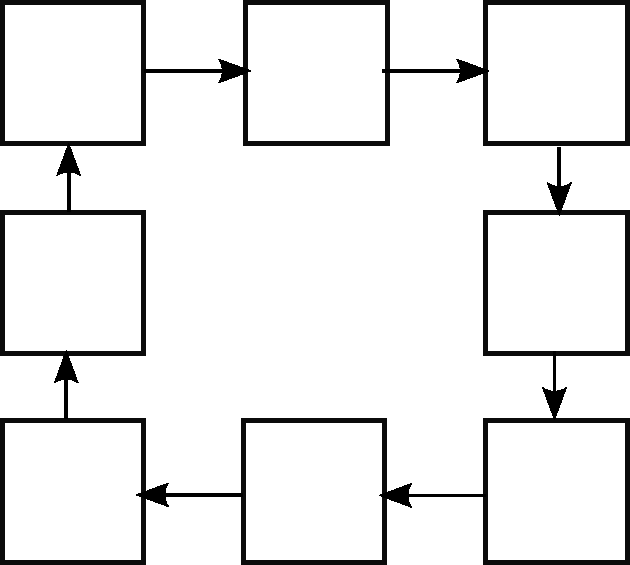
\includegraphics [scale=0.5]{colRot.pdf}

  \end{center}
  \caption{The rotation of one column shown apart from the shape. The active elements are considered to be part of the same layer.}
  \label{layer}
\end{figure}

In order to describe movement and orientation, a number of terms are used. This section provides a brief summary of their intended meaning.
\begin{itemize}
\item {\bf Row:} All blocks which share a common \emph{y} value. In addition, they should be equidistant from the \emph{z}-axis. This ensures that only blocks on the same `layer' are moved by controls affecting a single row. The active layer is always the outermost one (i.e. where at least one face of every cube in that row is visible). 
\item {\bf Column:} All blocks which share a common \emph{x} value. In addition, they should be equidistant from the \emph{z}-axis. This ensures that only blocks on the same `layer' are moved by controls affecting a single column. Figure~\ref{layer} illustrates what is meant by a `layer'. The active layer is always the outermost one (i.e. where at least one face of every cube in that column is visible).
\item {\bf \emph{x}-axis:} This axis is considered to run horizontally across the screen. 
\item {\bf \emph{y}-axis:} This axis is considered to run vertically along the screen. 
\item {\bf \emph{z}-axis:} This axis is considered to run perpendicular to the \emph{x}- and \emph{y}-axis. That is, it lies perpendicular to the surface of the screen, with the positive \emph{z} values coming out towards the user.
\item {\bf Origin:} The origin is defined as follows in relation to the overall \gls{shape}: \\
\emph{$Centre_x$} = Maximum length of \gls{shape} in \emph{x} $\div$ 2 \\
\emph{$Centre_y$} = Maximum length of \gls{shape} in \emph{y} $\div$ 2 \\
\emph{$Centre_z$} = Length of \gls{shape} in \emph{z} along the line that goes through point ($Centre_x$, $Centre_y$) $\div$ 2 \\
Thus, the origin is defined as ($Centre_x$, $Centre_y$, $Centre_z$).

\end {itemize}

\subsubsection{Controls}
\begin{figure}
  \centering
  \subfloat[Initial shape]{\label{fig:gull}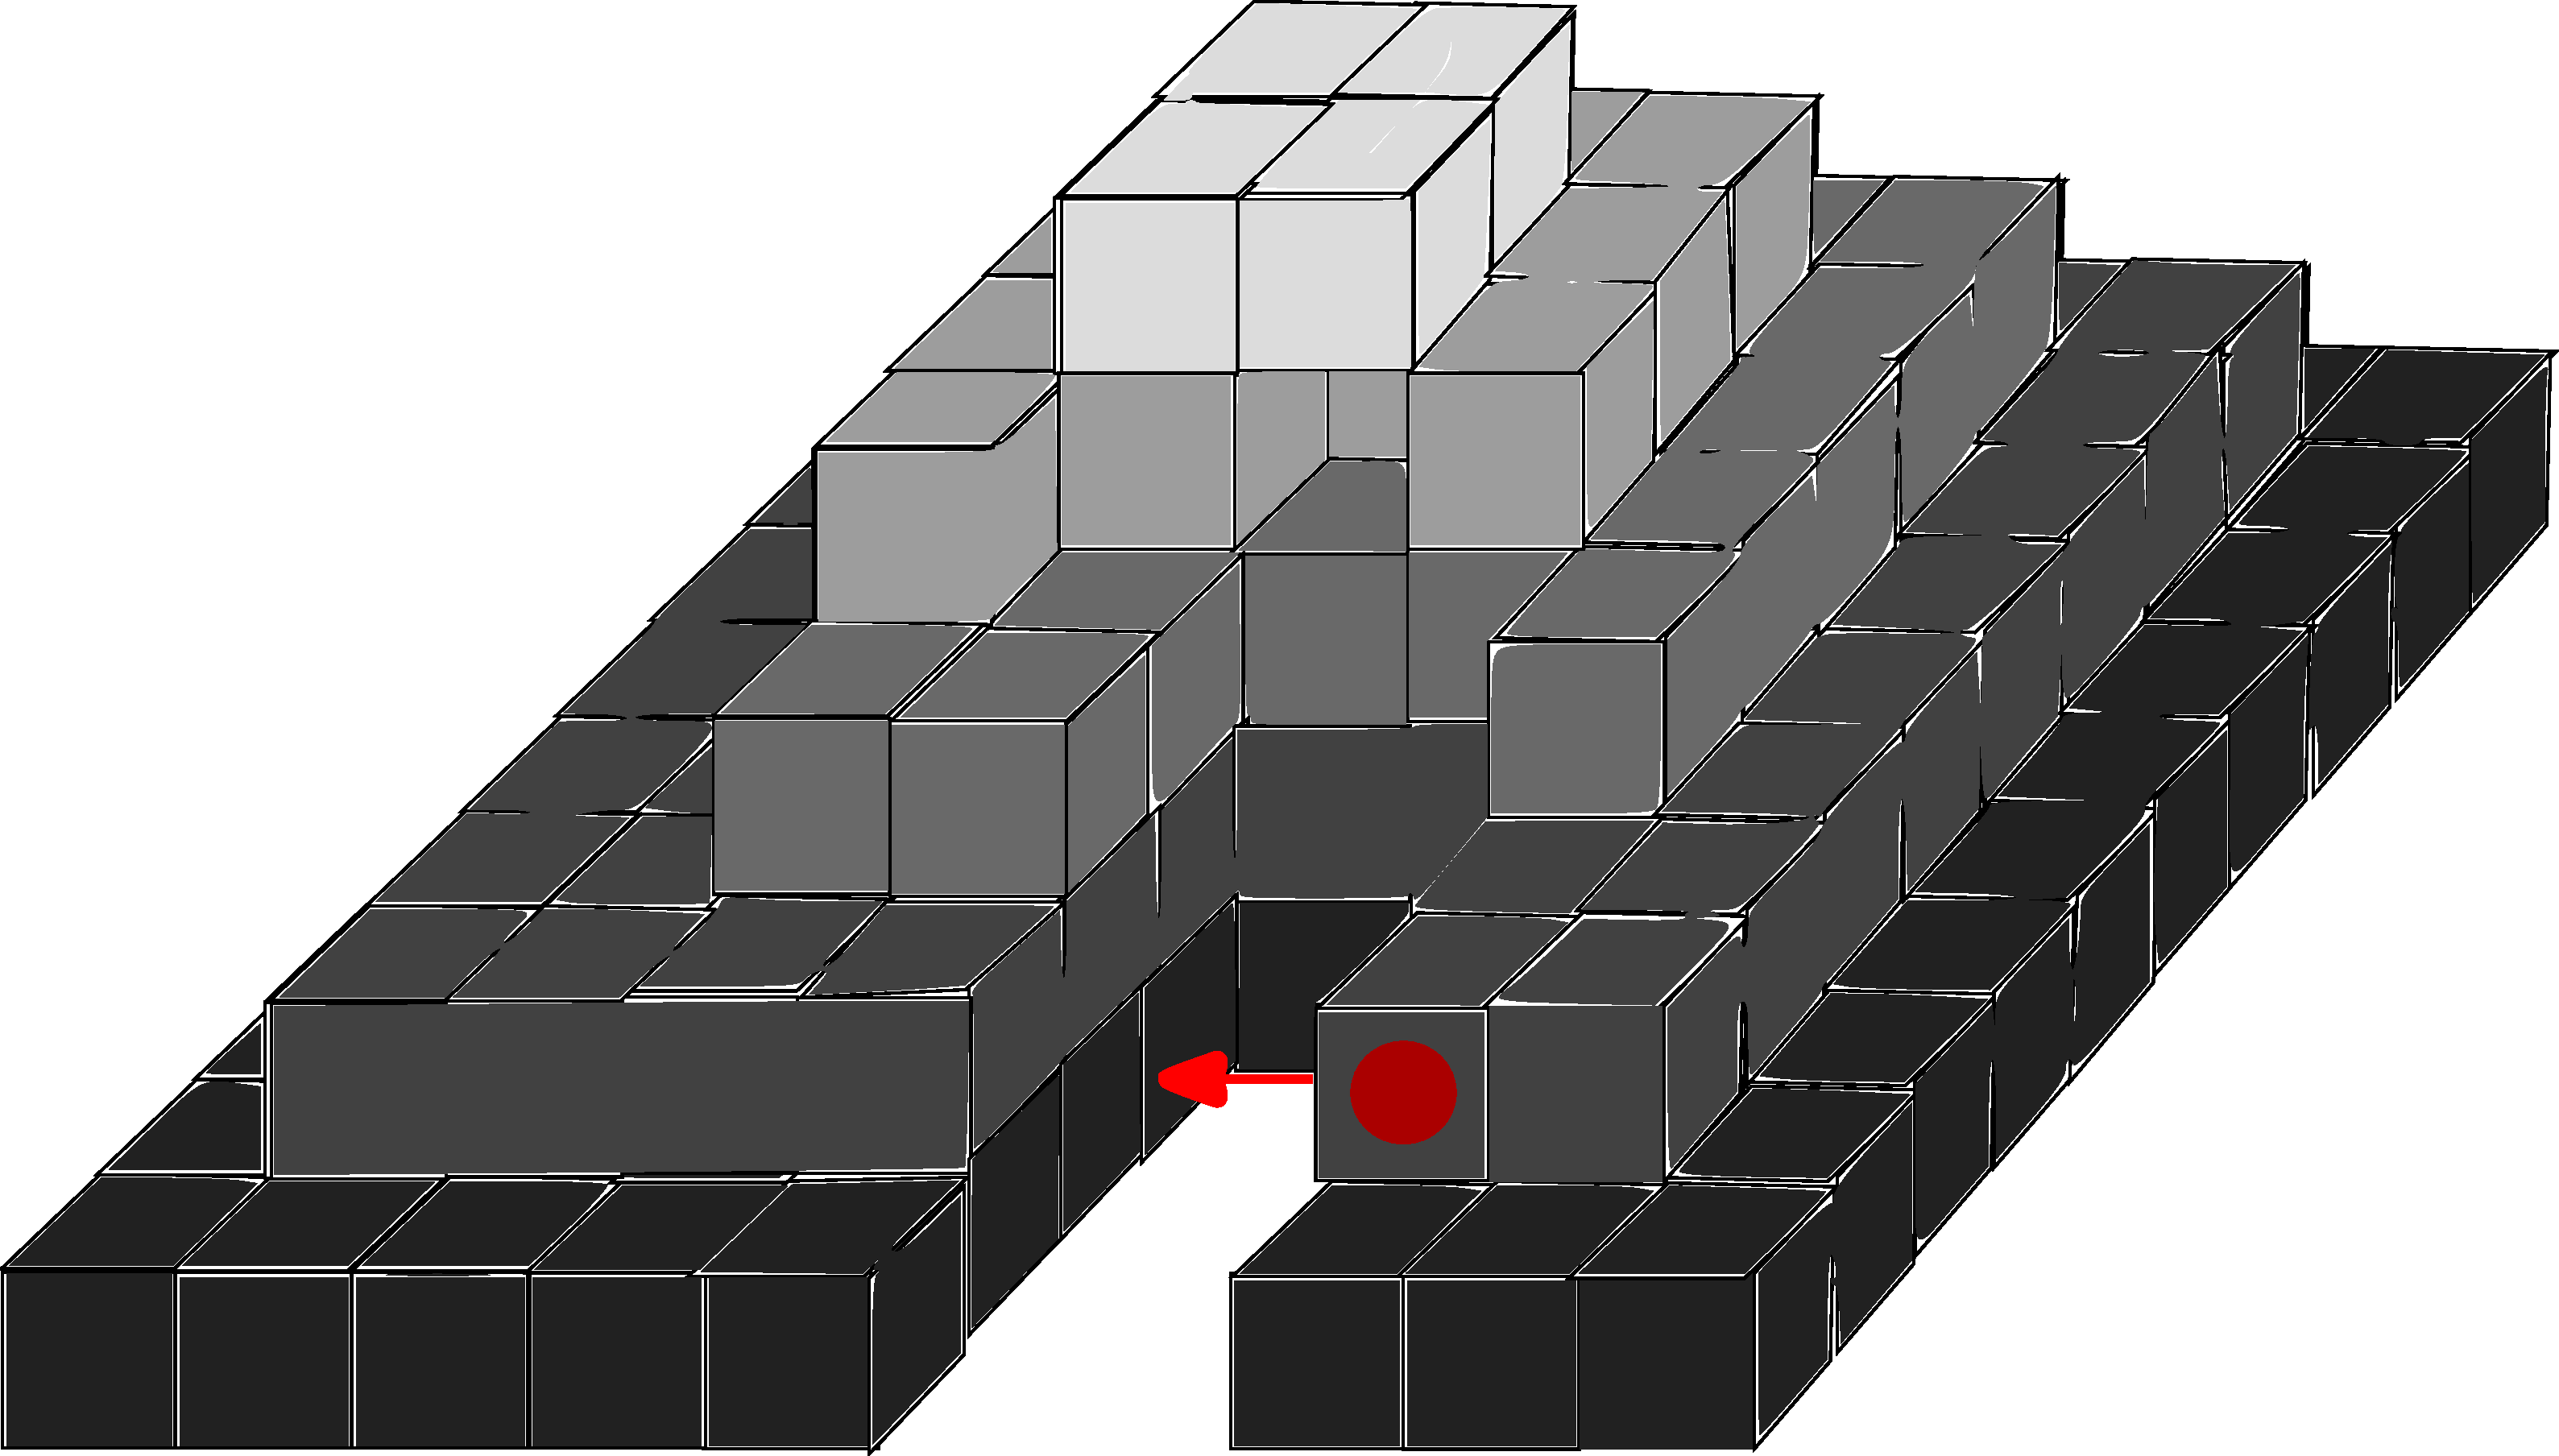
\includegraphics[scale=0.1]{left1.pdf}}       \hspace{20pt}          
  \subfloat[Shape after \emph{Left} gesture has been applied. The red dot indicates which block it was applied to, while the arrow shows direction of movement.]{\label{fig:tiger}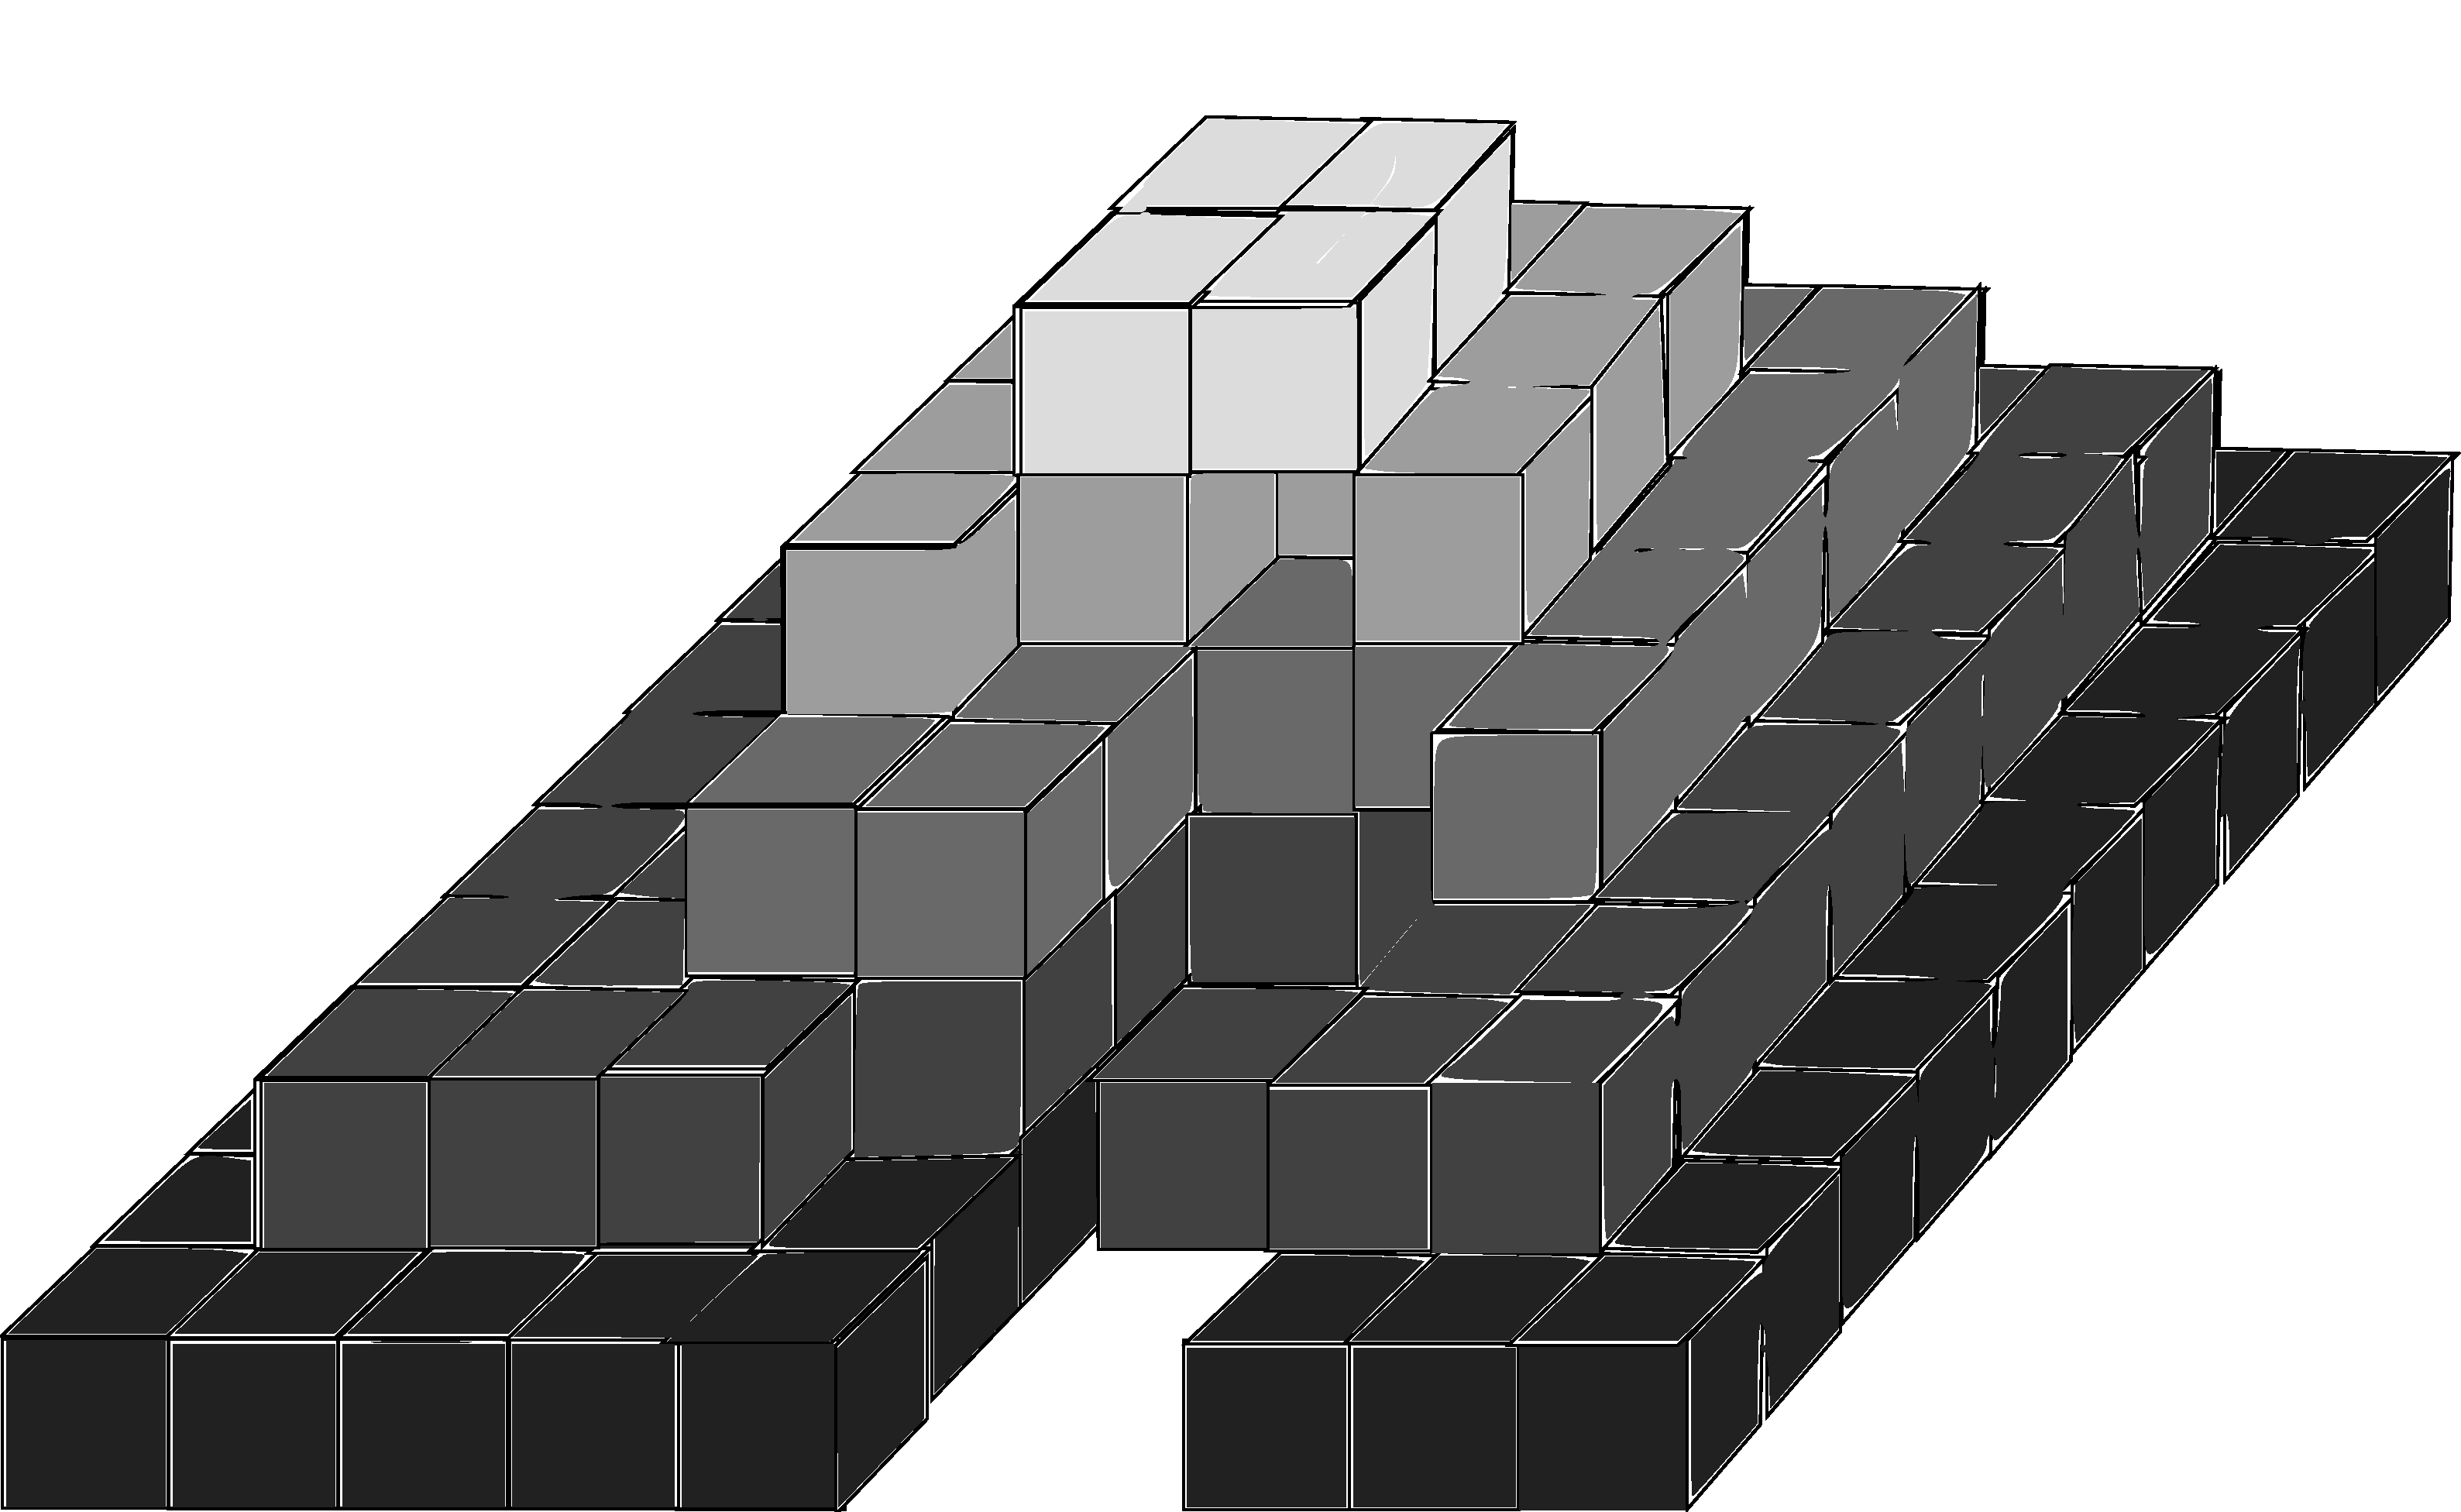
\includegraphics[scale=0.1]{left2.pdf}} \hspace{20pt}        
  
  \caption{Illustration of \emph{Left} gesture on the square pyramid with blocks missing.}
  \label{left}
\end{figure}

Cubes will be able to be arranged by means of controls that displace blocks with those around them in much the same way as is used in a \emph{Rubik's Cube}. That is, all cubes in a single row (blocks along the \emph{x}-axis with a constant value on the \emph{y}-axis) or column can be rotated around the relevant axis. An example of such rotations around the \emph{y}- and \emph{x}-axes are shown in Figure~\ref{left} and \ref{upTwo}. In addition, cubes will be able to be swapped with the cubes below or above them (on the \emph{z}-axis) as well. Finally, controls for removing any gaps that may have been caused by block removal as well as slightly rocking the \gls{shape} (so as to give an impression of three-dimensionality) will also be included. These controls were decided upon as they provide a maximum amount of control while only requiring minimal learning from the player. That is, as many of the controls are just variations of the same idea, but in different directions, a player only has to grasp and remember a small number of movement techniques. This, in turn, reduces the cognitive load placed on the player~\citep{Niel04}. A \emph{New game} button will also be included in case the user wants to begin a new game or can no longer execute any significant movement commands.

\begin{figure}[h]
  \centering
  \subfloat[Initial shape with missing blocks.]{\label{fig:gull}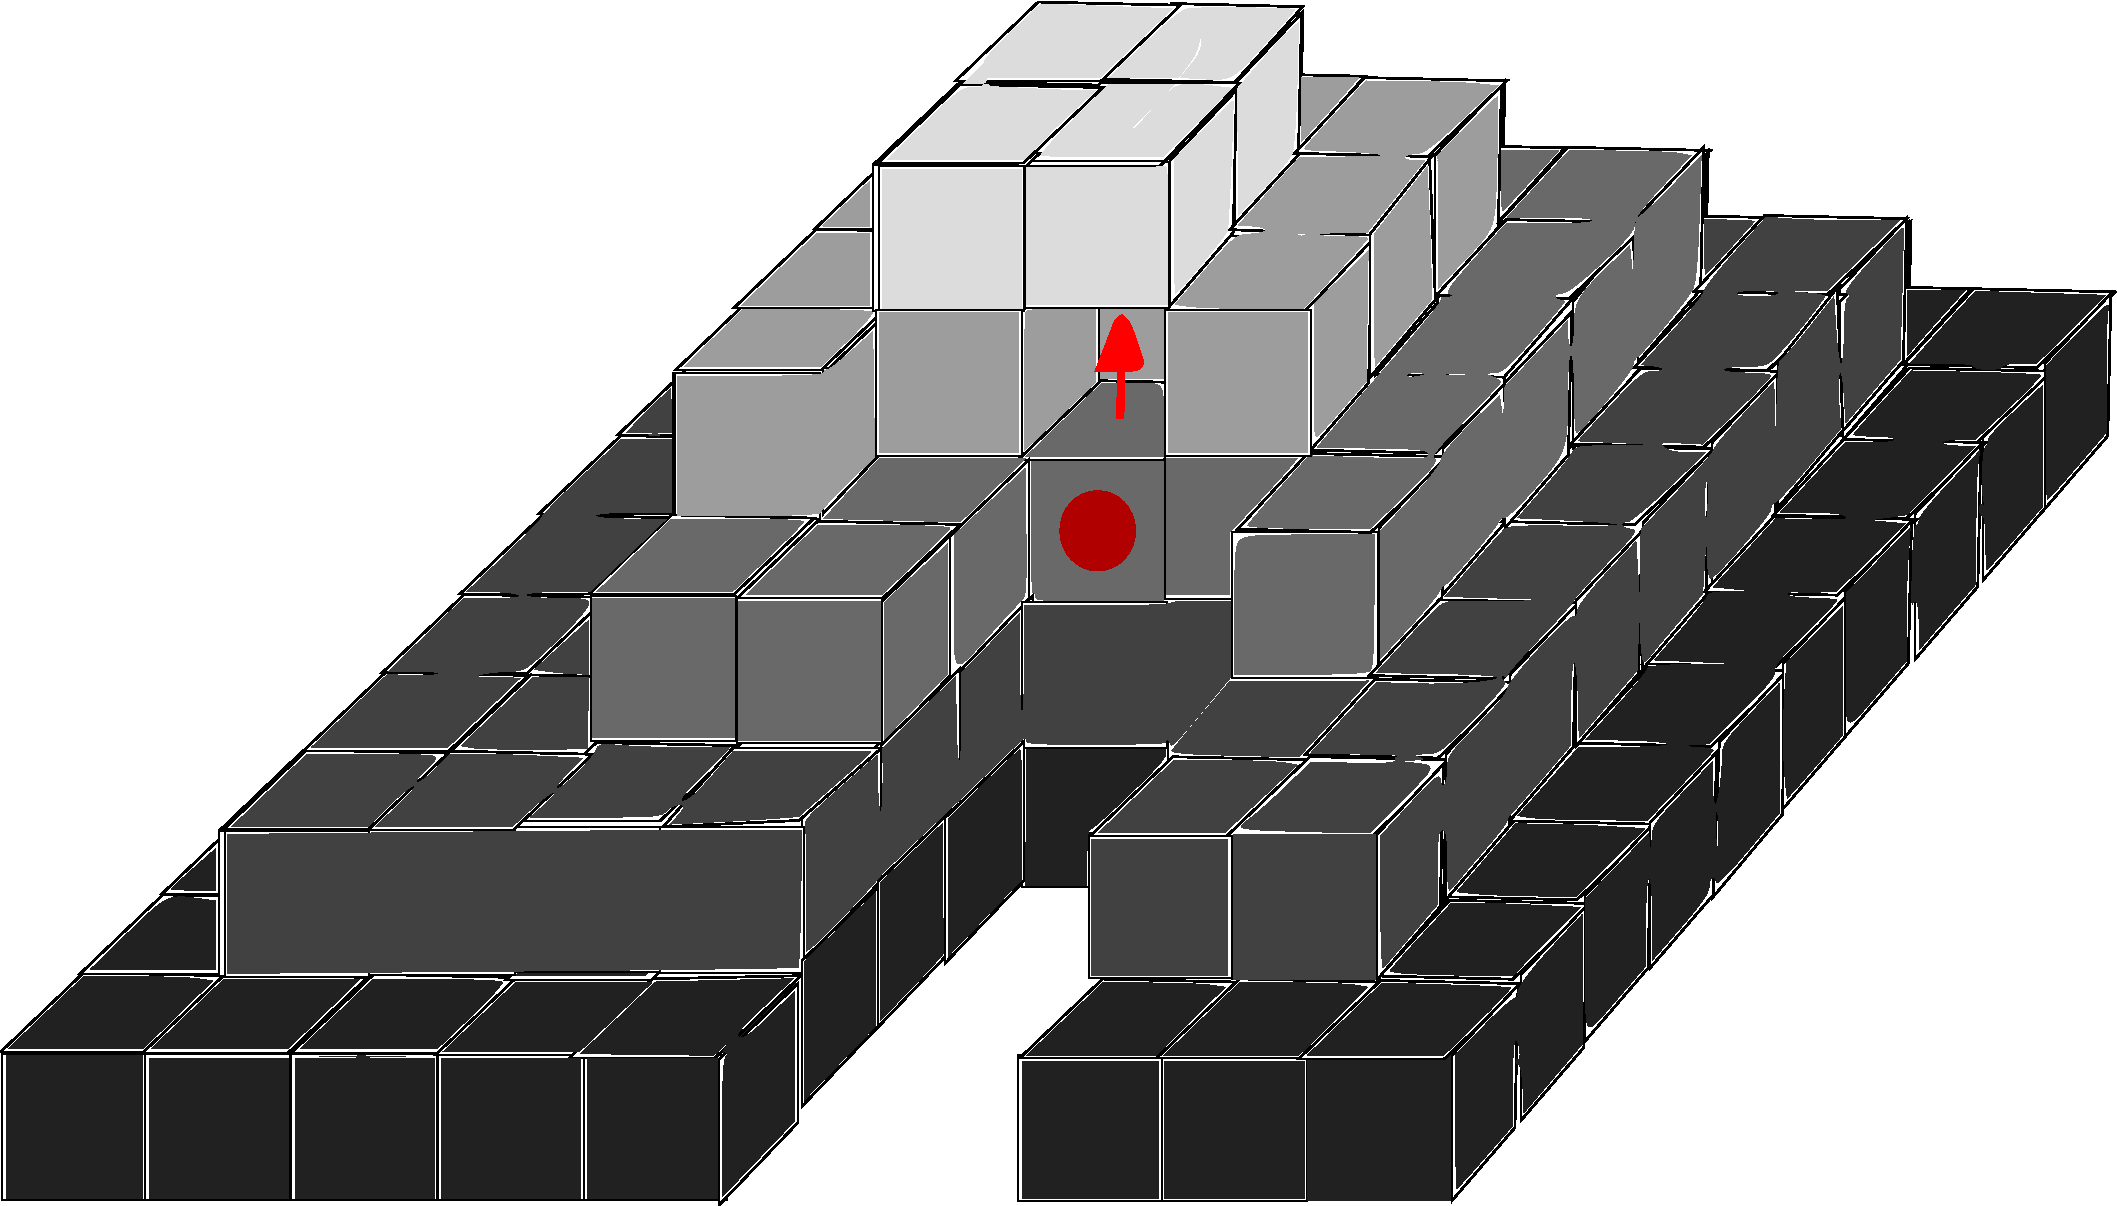
\includegraphics[scale=0.1]{up_1.png}}       \hspace{20pt}          
  \subfloat[Shape after \emph{Up} gesture has been applied. The red dot indicates which block it was applied to, while the arrow shows direction of movement.]{\label{fig:tiger}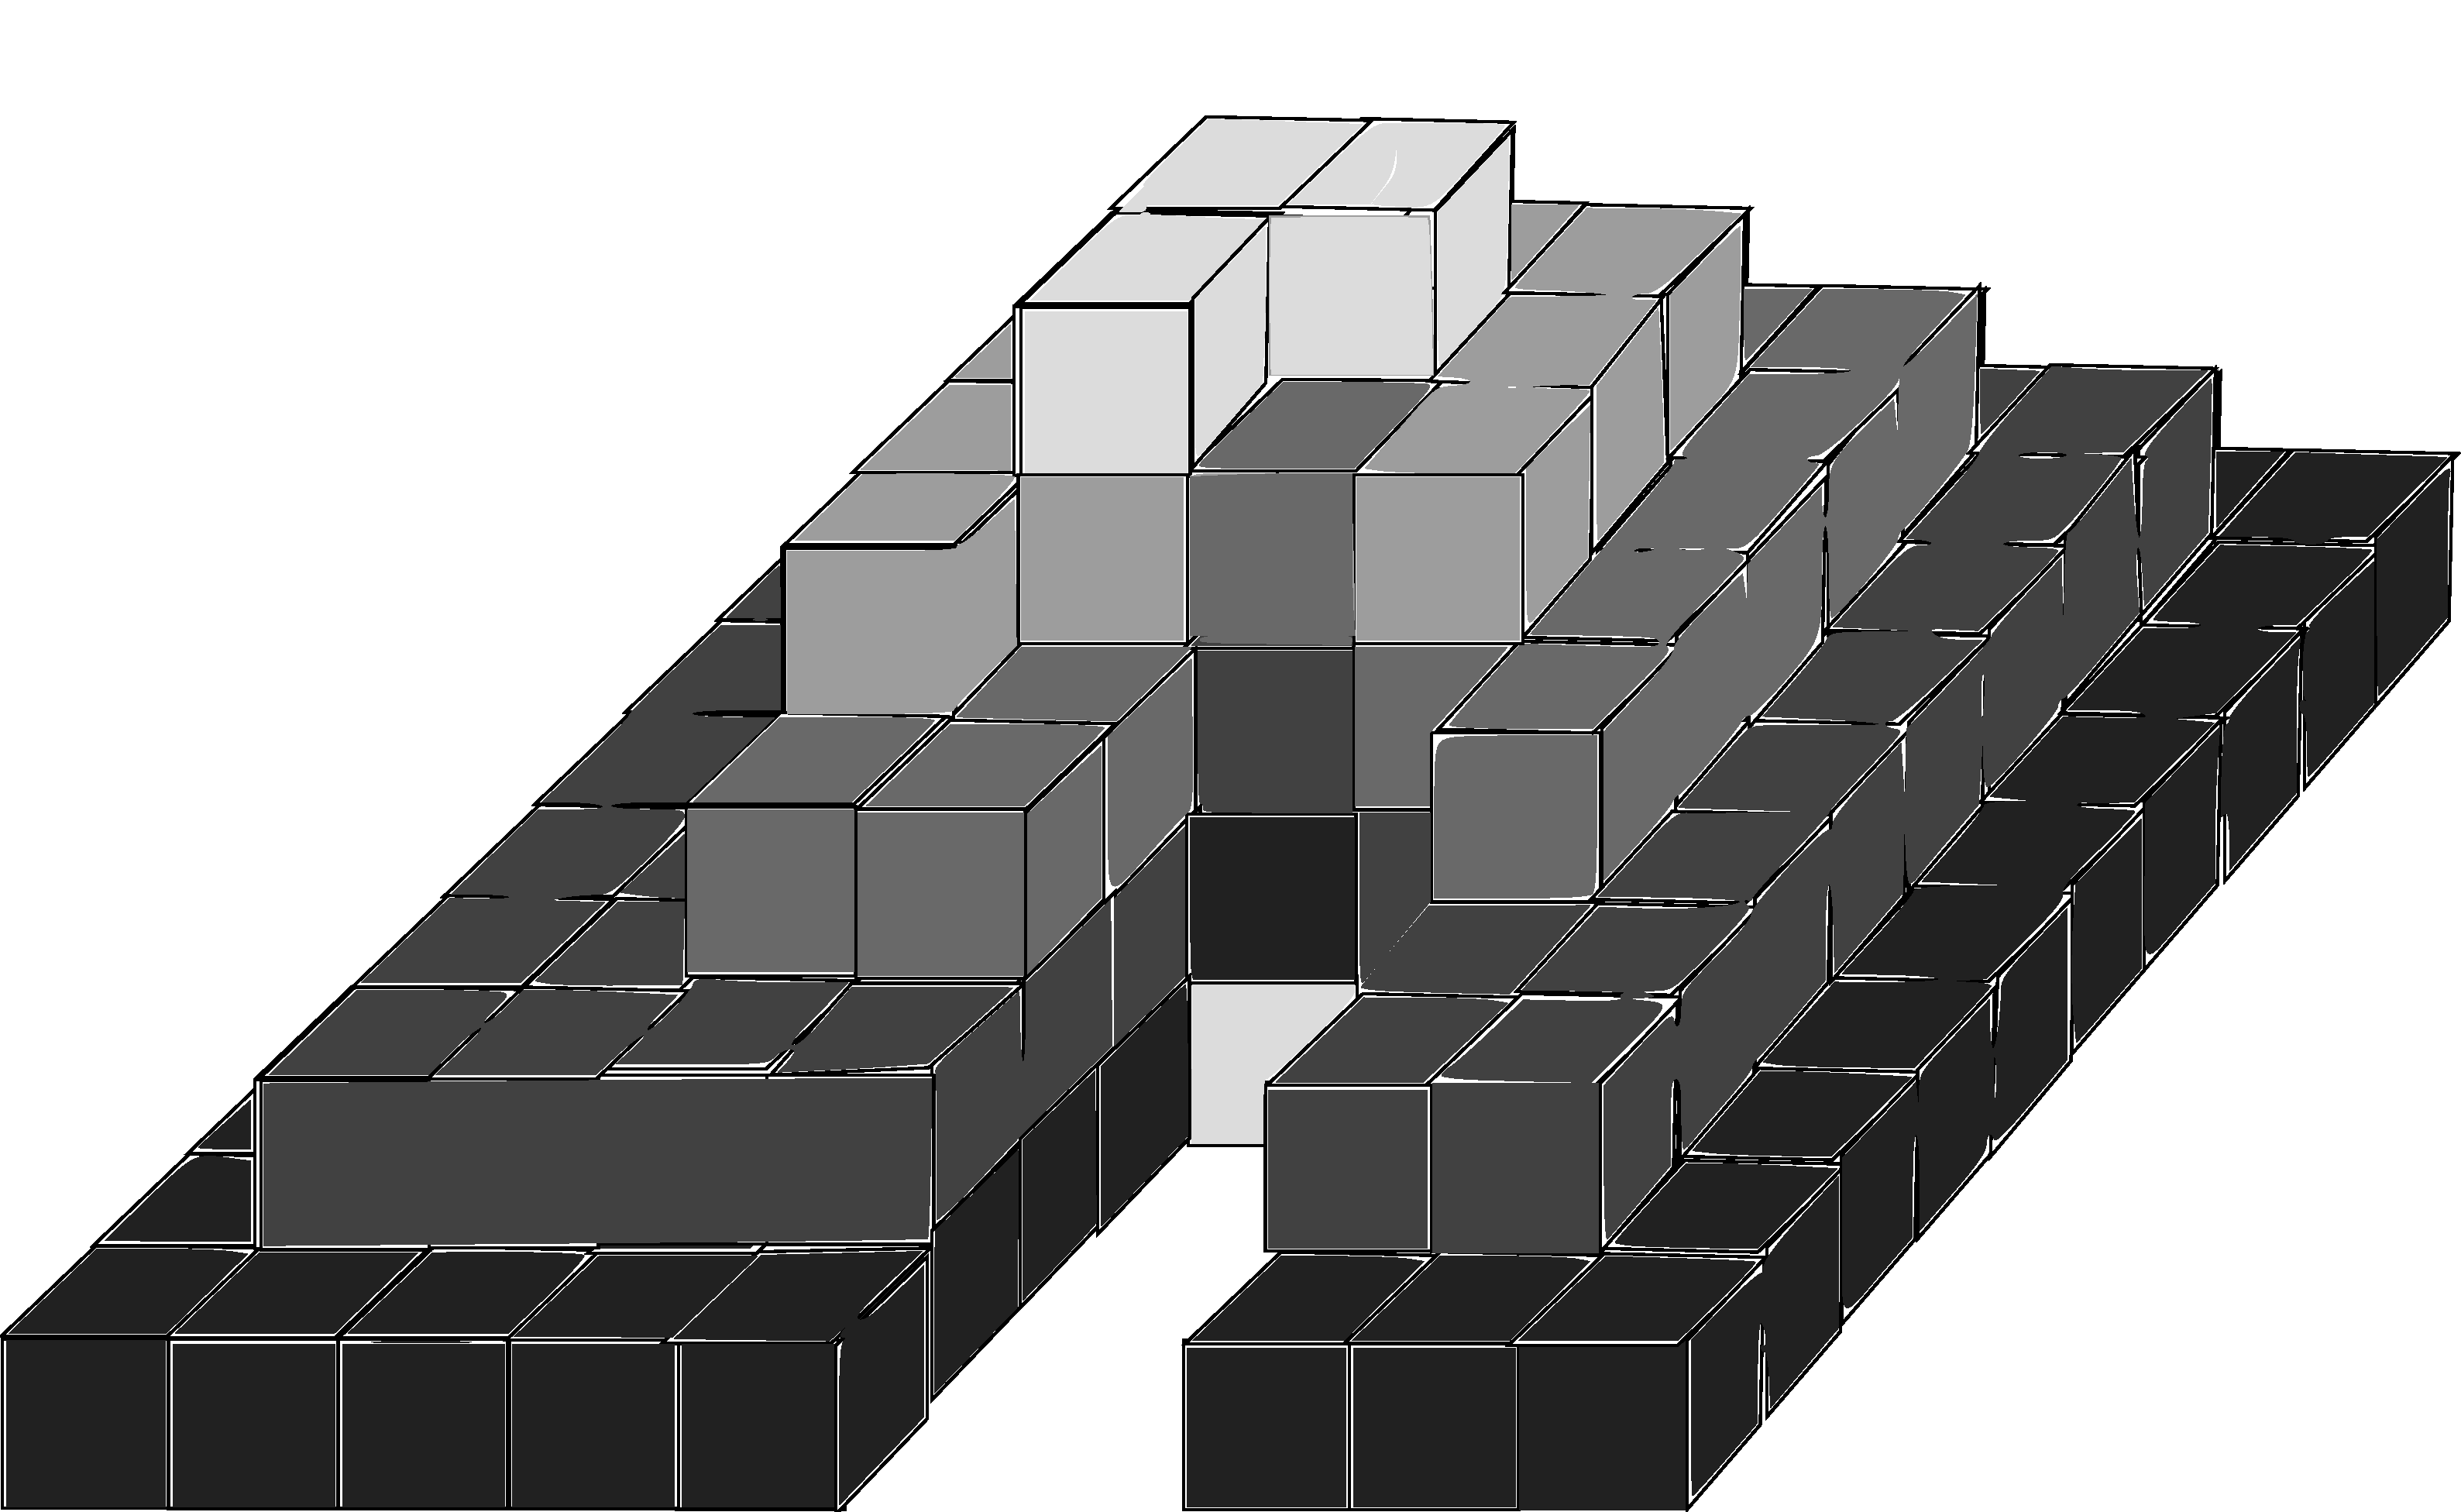
\includegraphics[scale=0.1]{up_2.pdf}} \hspace{20pt}        
  
  \caption{Illustration of \emph{Up} gesture on the square pyramid with blocks missing. The red dot indicates which block it was applied to, while the arrow shows direction of movement.}
  \label{upTwo}
\end{figure}

\begin{figure}
  \centering
  \subfloat[Initial shape]{\label{fig:gull}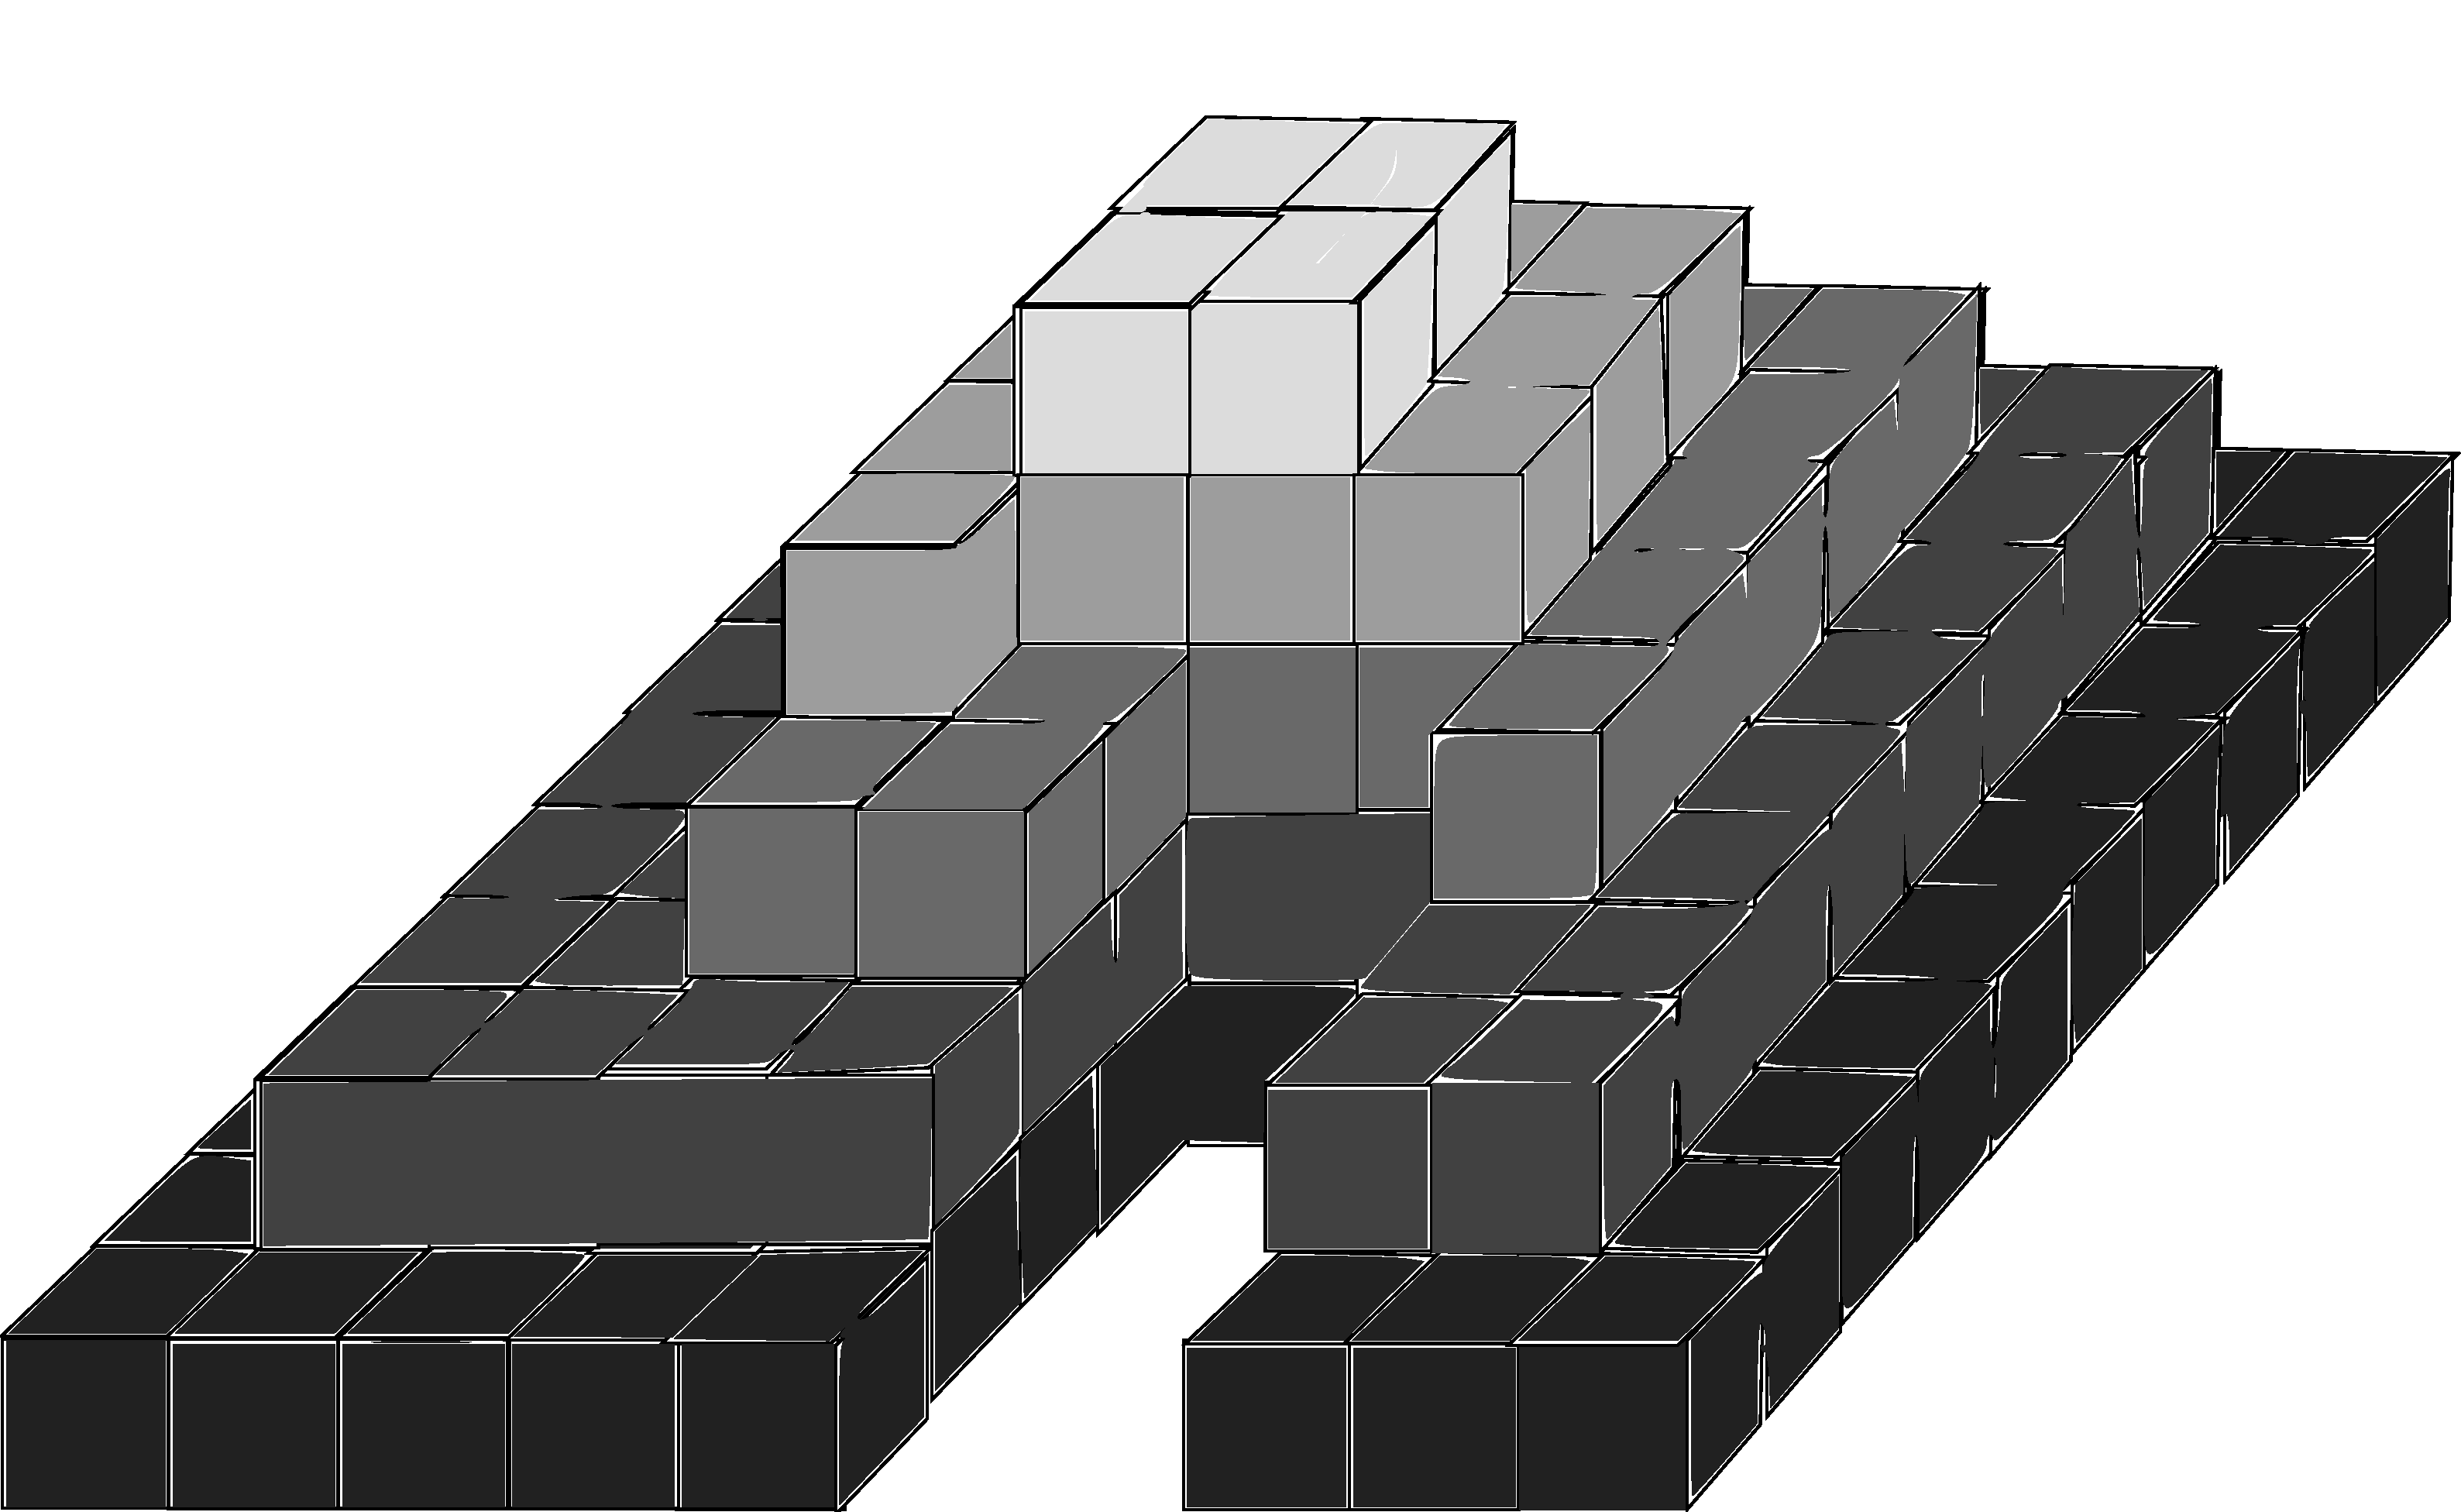
\includegraphics[scale=0.1]{gaps1.pdf}}       \hspace{20pt}          
  \subfloat[Shape after \emph{Fill in the gaps} gesture has been applied.]{\label{fig:tiger}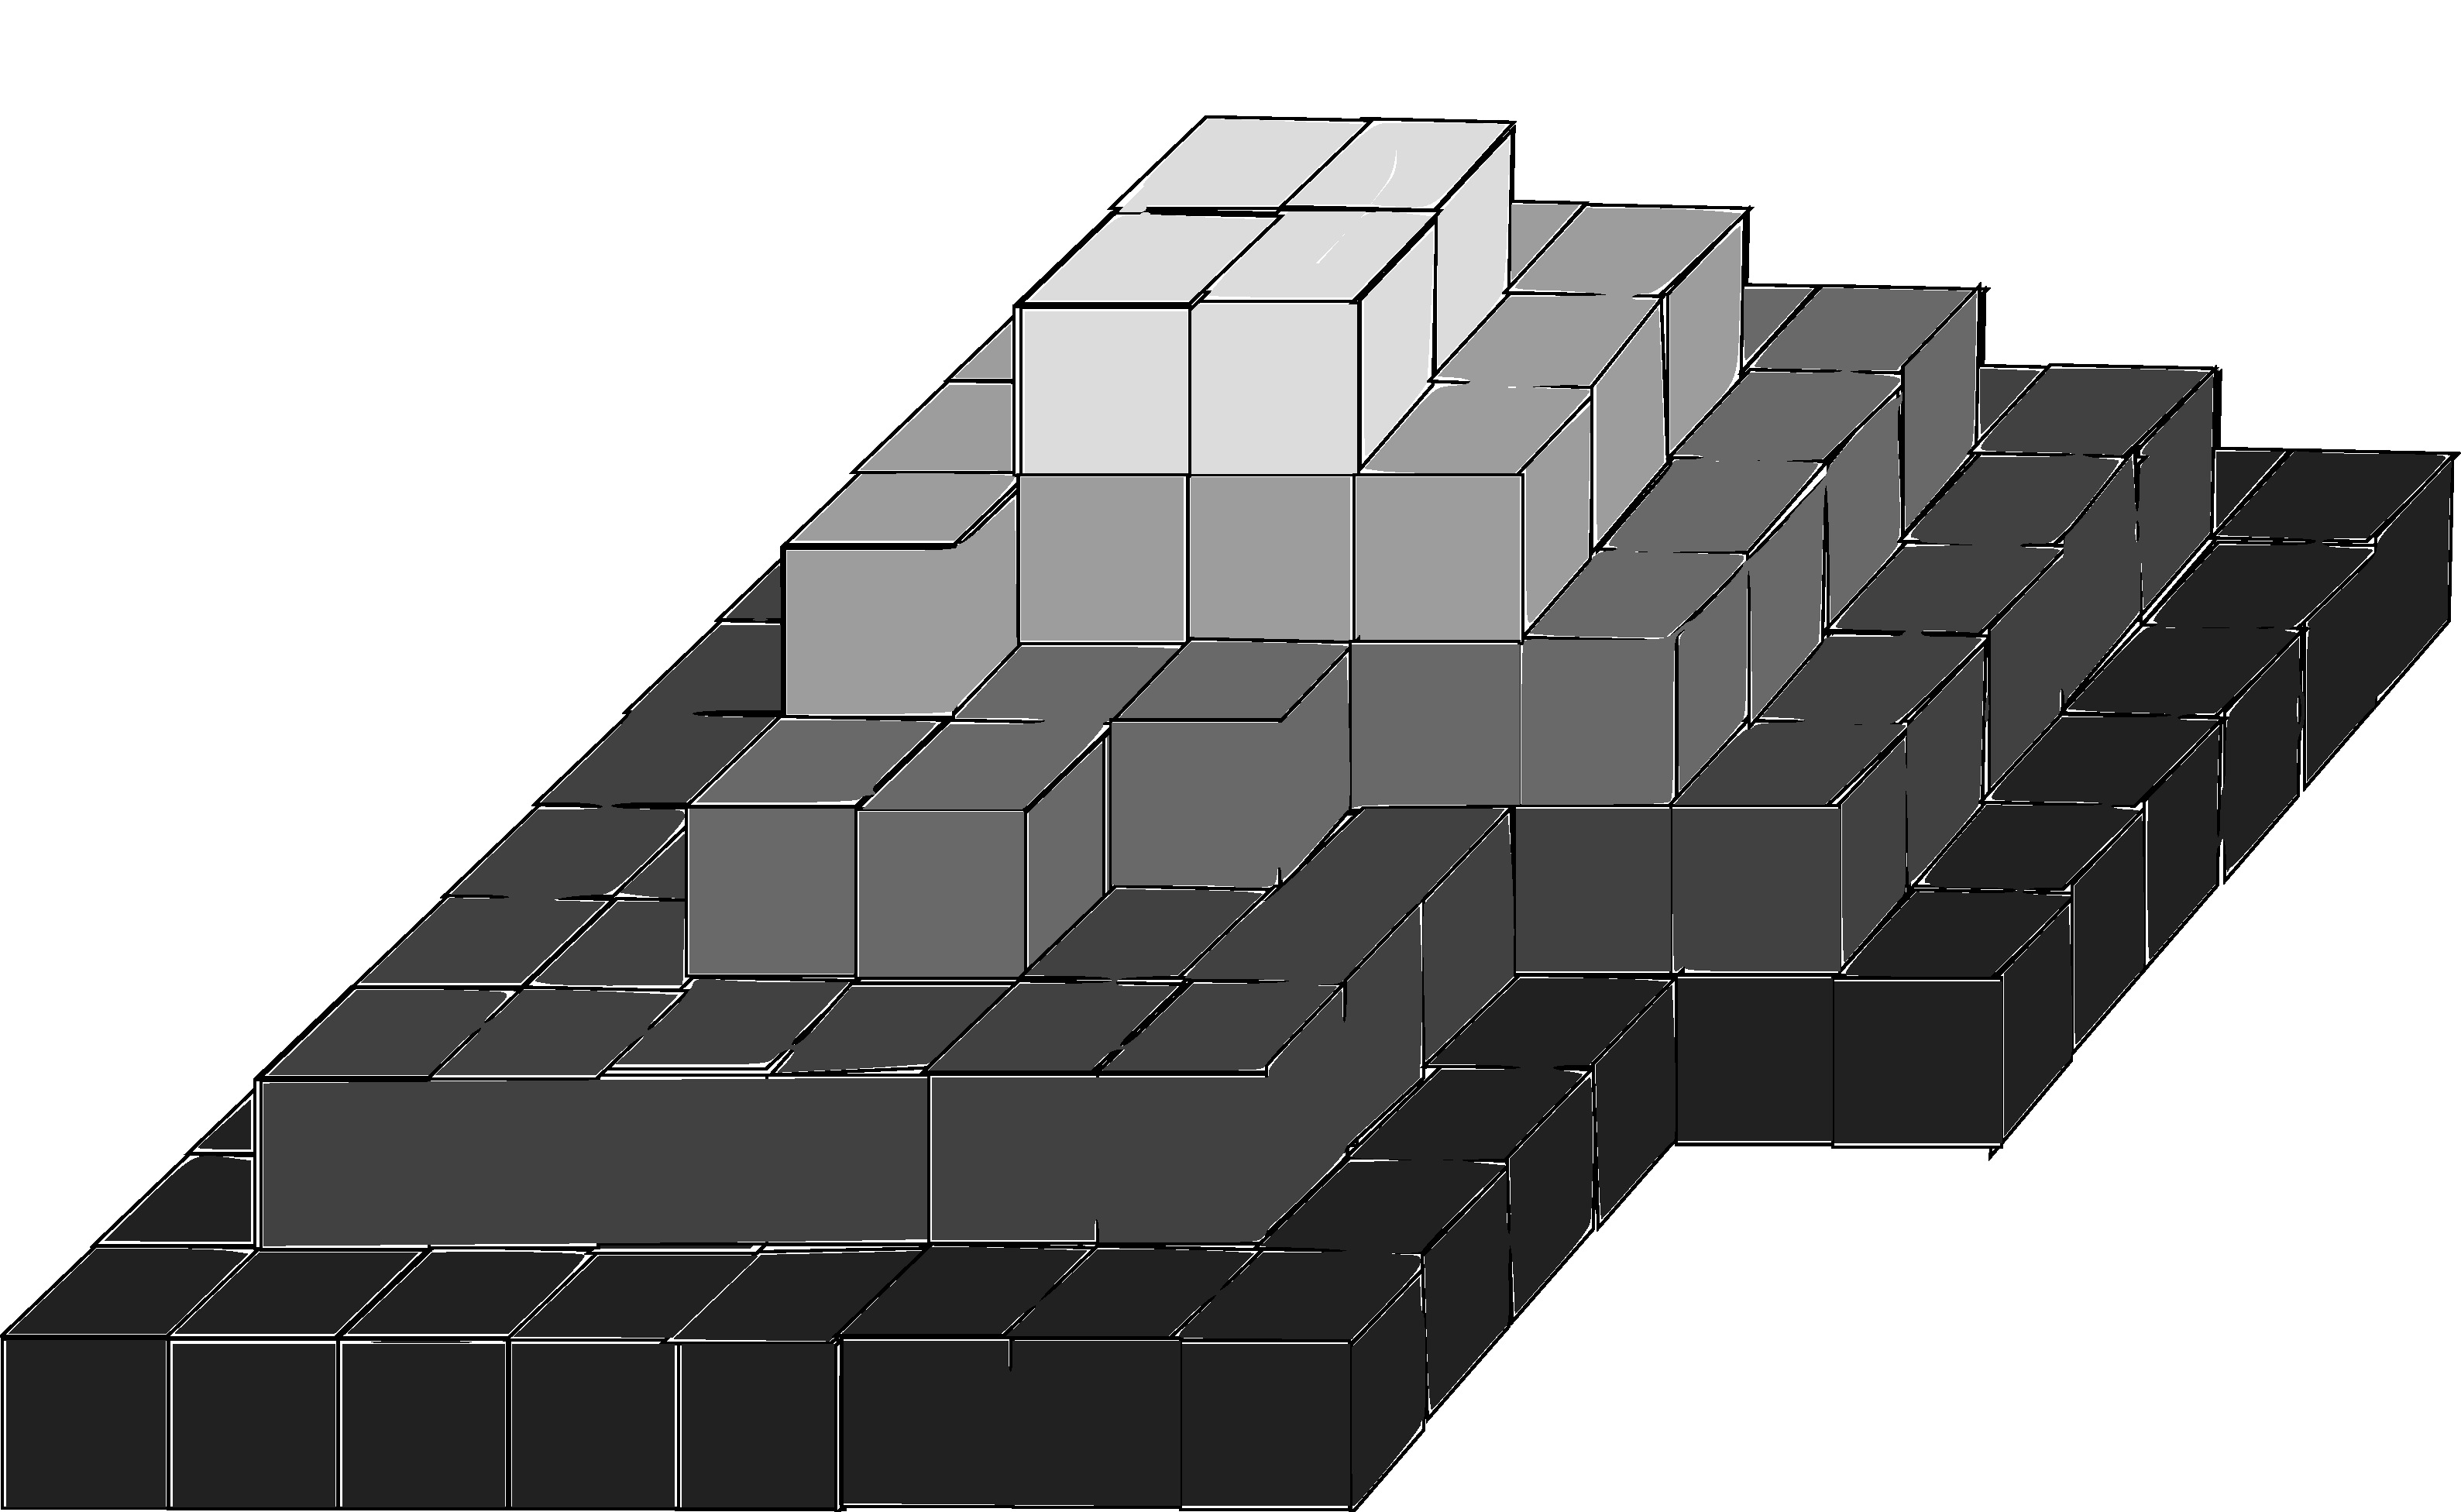
\includegraphics[scale=0.1]{gaps2.pdf}} \hspace{20pt}        
  
  \caption{Illustration of \emph{Fill in the gaps} gesture on the square pyramid with blocks missing.}
  \label{gaps}
\end{figure}

\paragraph{Gestural interface}
Gestures will be used to control block manipulations. In order to apply a specific action to cube, the player will need to begin that gesture on the required cube. This removes the need for extra taps in order to determine the target of each gesture. It also utilises the context-sensitivity possible with gestural interaction~\citep{Wobb09}. Gestures were chosen so that they provided some form of affordance to the player. That is to say that their form could logically be linked with their action. This is of importance as gestures do not provide the same affordances as more traditional, button-based interfaces~\citep{Niel04}. This in turn may mean that users are required to memorise a far greater number of commands. By making gestures logically relateable to their purpose, one can lessen this memory load~\citep{Jaim07}. In addition, gestures that applied the same movement technique, but in different directions, were created from variations of a single model. This too was done to reduce cognitive requirements placed on the player~\citep{Niel04}.

A full list of possible moves as well as their descriptions are provided in Table~\ref{gestureList}. A dot indicates the beginning of the gesture in order to show directionality. 
\begin{table}
\centering %
\begin{tabular*}{\textwidth}{p{2cm} p{7cm} p{3cm} p{1cm}}
\hline
Movement type & Description & Number of blocks affected & Diagram\\\hline
Left & Rotate all blocks in a row left around the \emph{y}-axis by one place. & One row &\begin{center}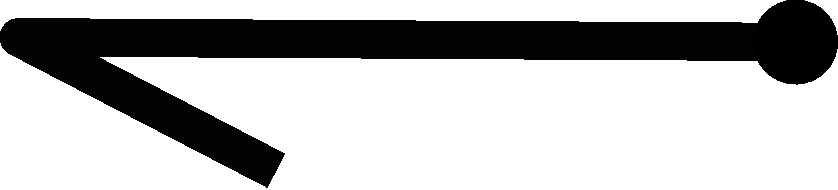
\includegraphics [width=1.5cm]{left.pdf}\end{center} \\
Right & Rotate all blocks in a row right around the \emph{y}-axis by one place. & One row &\begin{center}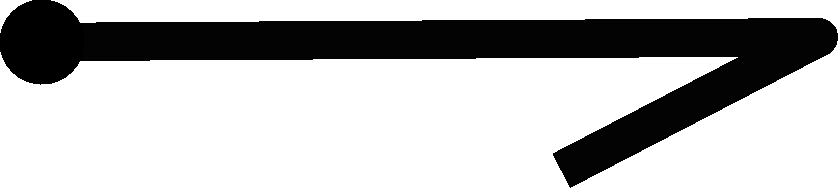
\includegraphics [width=1.5cm]{right.pdf}\end{center} \\
Up & Rotate all blocks in a column up around the \emph{x}-axis by one place. & One column &\begin{center}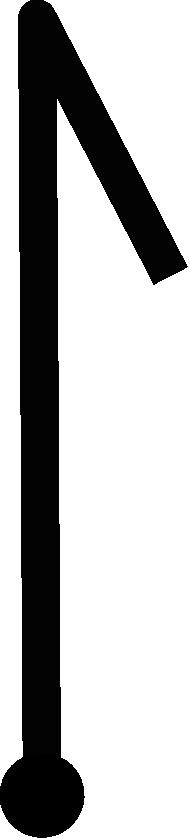
\includegraphics [height=1.5cm]{up.pdf}\end{center} \\
Down & Rotate all blocks in a column down around the \emph{x}-axis by one place. & One column &\begin{center}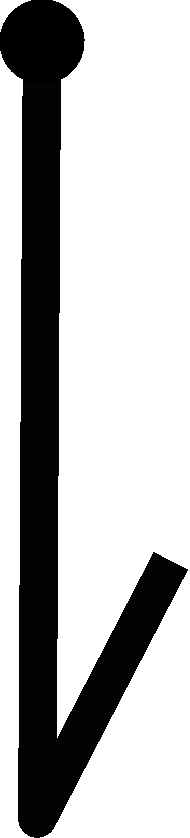
\includegraphics [height=1.5cm]{down.pdf}\end{center} \\
Forward & Move all blocks on one line along the \emph{z}-axis forward by one place. The forward-most block moves to the back of the shape. & One line along the \emph{z}-axis &\begin{center}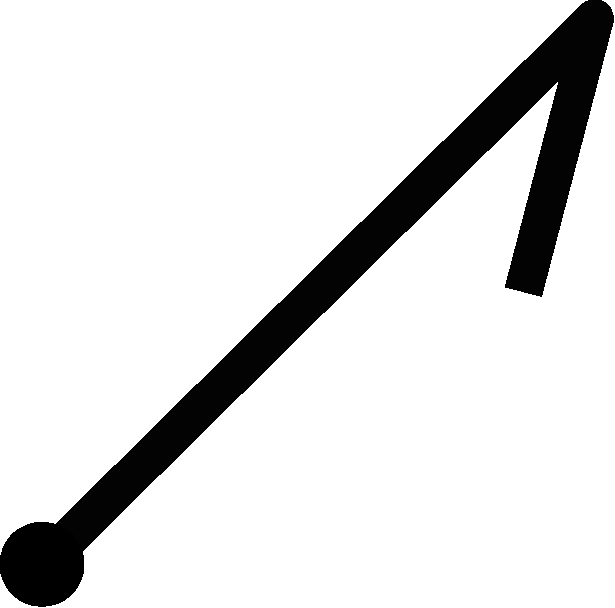
\includegraphics [scale=0.1]{forward.pdf}\end{center} \\
Backward & Move all blocks on one line along the \emph{z}-axis backward by one place. The backward-most block moves to the front of the shape. & One line along the \emph{z}-axis &\begin{center}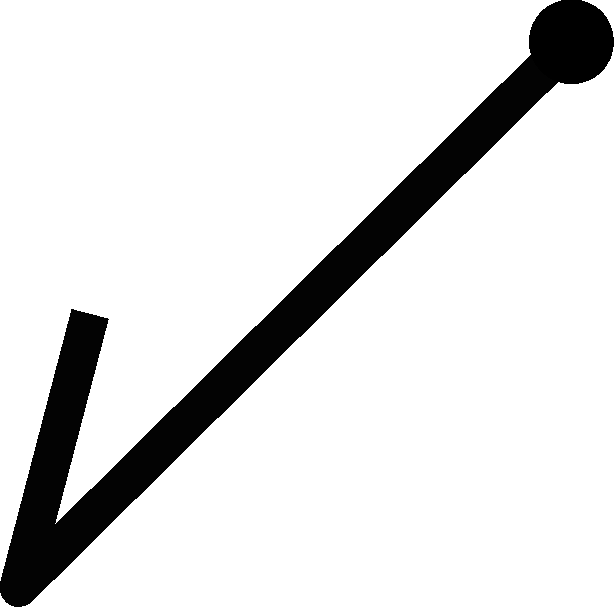
\includegraphics [scale=0.1]{backward.pdf}\end{center} \\
Fill in gaps & Move all blocks that have an equal distance from the origin (i.e. one `level' of the shape) together, filling in any gaps that may have been caused by removing blocks. This action is demonstrated in Figure~\ref{gaps}. & All blocks of a certain distance from the origin &\begin{center}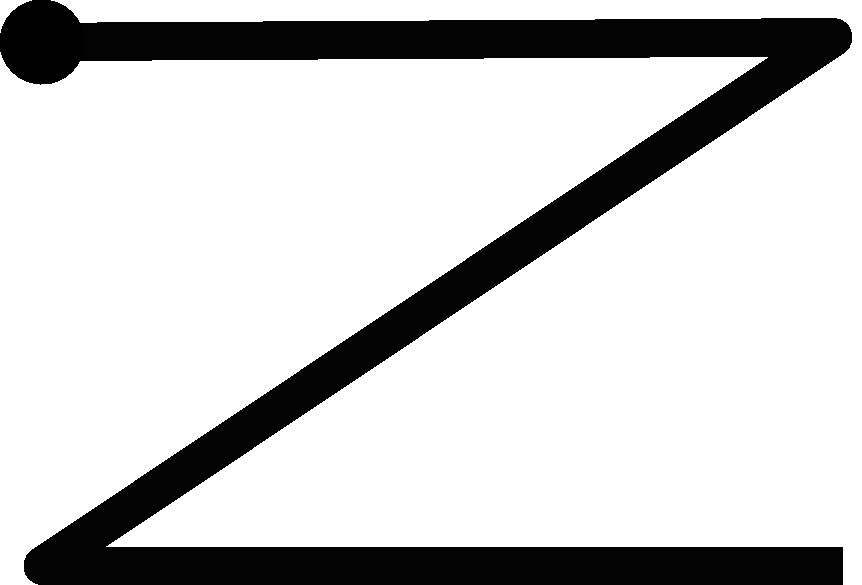
\includegraphics [scale=0.1]{z.pdf}\end{center} \\
Swap & Swaps two blocks with each other. The direction the swap is performed is chosen by using one of the gestures for Left, Right, Up, Down, Backward or Forward without the preceding line. & Two neighbouring blocks &\begin{center}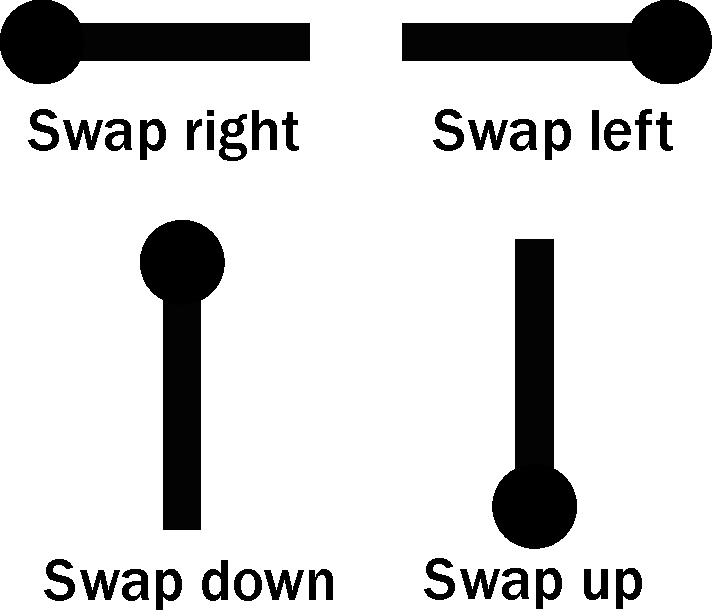
\includegraphics [scale=0.15]{swap.pdf}\end{center} \\
Rock & This repeatedly tilts the \gls{shape} slightly so that the player has a chance to see the surrounding faces of the shape. & All blocks &\begin{center}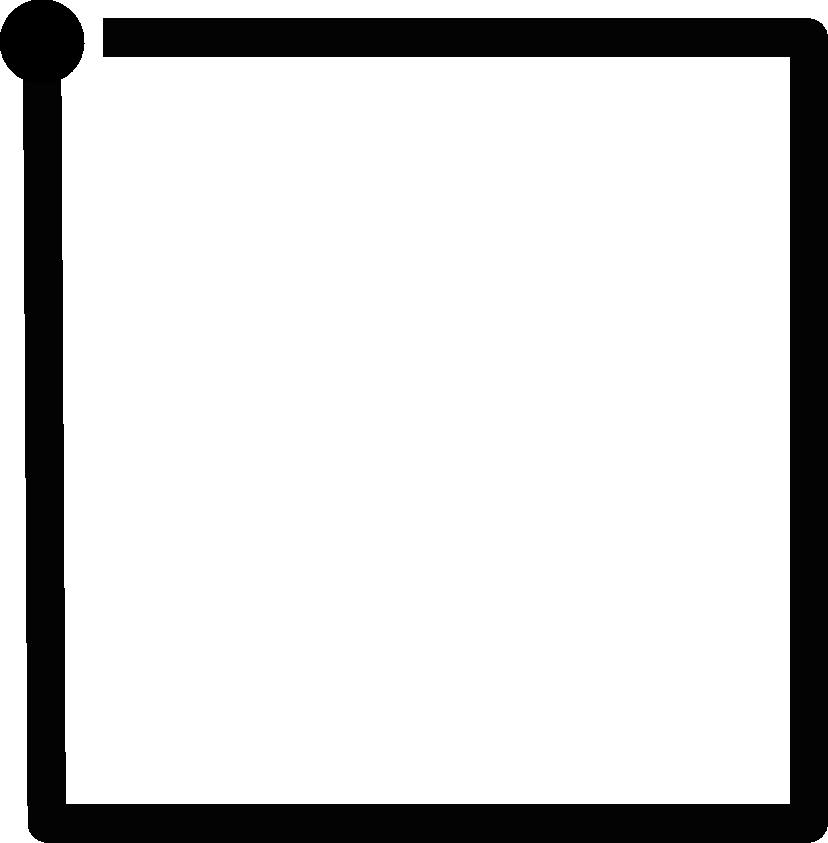
\includegraphics [scale=0.1]{rock.pdf}\end{center} \\
\hline 
\end{tabular*}
\caption{Description and illustration of all gestures that will be used in the game. The black dot indicates the start point of the gesture.}
\label {gestureList}
\end{table}
Block removals will be done by tapping the required block. Gaps left by removing blocks will remain until the user applies a \emph{Fill in gaps} command.

\paragraph{Direct manipulation version}

The direct manipulation version will have the same functionality as the gestural game. However, all controls will take the form of buttons displayed on the side panel which displays hints in the gestural version. Rotation will also be implemented by means of buttons in order to maintain consistency and not confuse the user. In order to use the controls that relate to specific blocks, a player will be required to select the appropriate control. They are then able to apply the movement by selecting blocks. When a movement control has a number of variants (for example, \emph{Left}, \emph{Right} and so on) a second sub-menu will be shown on the side of the main menu. This sub-menu will display the variants so as not to clutter the main menu. The selected control will remain selected until the user either deselects it or selects a different control. This means that any interaction with the \gls{shape} will be interpreted as applying the selected movement control. This persistence of a selected command was chosen so that users who wish to apply a movement technique multiple times do not become frustrated with the number of menu selections they need to perform. An example of what such a menu will look like is provided in Figure~\ref{dmVersion}
\begin{figure}
  \begin{center}
    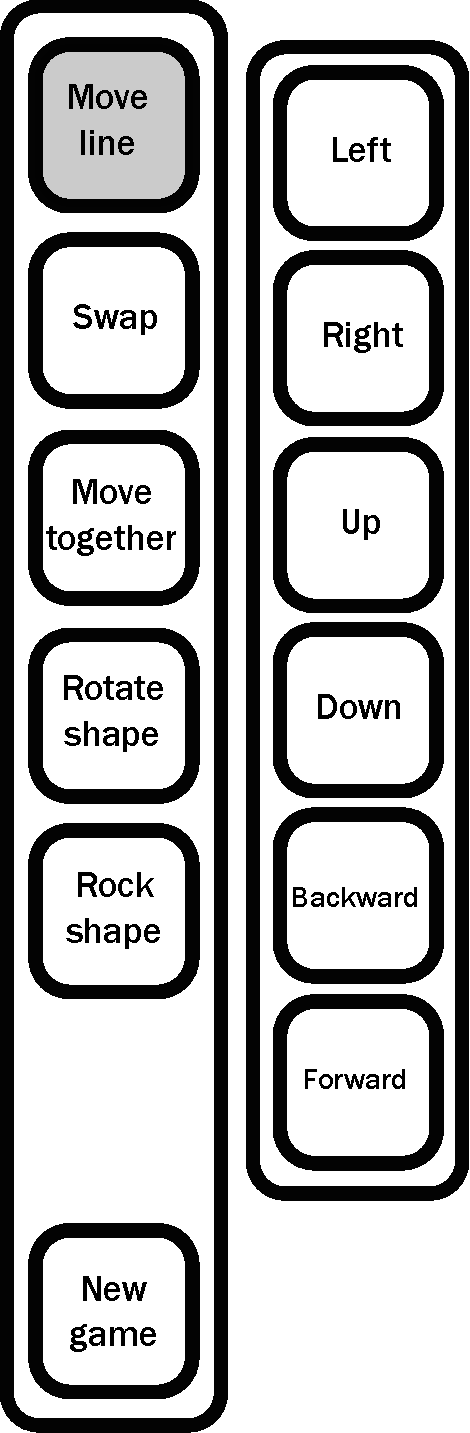
\includegraphics [scale=0.25]{dmVersion.pdf}

  \end{center}
  \caption{An example of the direct manipulation menu structure. As can be seen, when selecting an option with multiple variants, a second sub-menu is displayed.}
  \label{dmVersion}
\end{figure}

\paragraph{Mixed interface}
A combination of the two previous interface versions will be used in the mixed interface. That is, controls will be implemented through the use of both gestures and buttons. Gestural controls will be used for rotating rows and columns, moving blocks forwards or backwards along the \emph{z}-axis, swapping blocks and rotating the \gls{shape}. These commands were selected for gestural interpretation as they hold a strong logical correspondence to their action. In addition, all the commands represent only three underlying movement techniques (that of rotating the shape, swapping two blocks or moving a number of physically related blocks). The inclusion of both of these elements in a gestural form should reduce cognitive and memory requirements placed on the user. This, in turn, is expected to increase the effectiveness of their use~\citep{Niel04}. Buttons will be used to move blocks together in order to fill in the gaps as well as to rock the shape. These commands and their related gestures do not bear as much of a logical connection and thus were selected for button implementation as it may be found that this is more appropriate. Two disconnected menus will be placed on the left-hand side of the screen. The first will contain the buttons for manipulating the shape while the second will hold the appropriate subsection of the gesture hint panel.

\subsubsection{Removing blocks}
Cubes can be removed from the game by means of tapping a \gls{grouped}. If there are more than three neighbouring cubes of the same colour, they will be removed. Points are scored depending on how many blocks are removed at one time. Blocks can be linked together in any of the three dimensions, so long as at least one side is touching another block of the same colour.

When a \gls{grouped} removal has caused there to be spaces between a block and the other blocks comprising the \gls{shape}, the block will not be automatically moved to fill these gaps. Instead a gesture has been provided so that the player can choose whether to apply this effect. This is done so that players can strategically arrange blocks without having to take into account movement caused by removed blocks as this may be difficult to predict due to the three-dimensional nature of the shape.

\subsection{Target audience}
The demographic characteristics of the target market are fairly broad, as anyone who enjoys spatial thinking or puzzle-type games would be able to play. In addition, the puzzle market is not generally geared towards a specific age group or gender, allowing for a more diverse audience. The platform that will be used, however, does limit the target audience. As \emph{Hexahedron} will be developed for the iPad, the primary target market of the game will thus be individuals who own such a device and enjoy puzzle games.


\subsection{Design}
\begin{figure}
  \begin{center}
    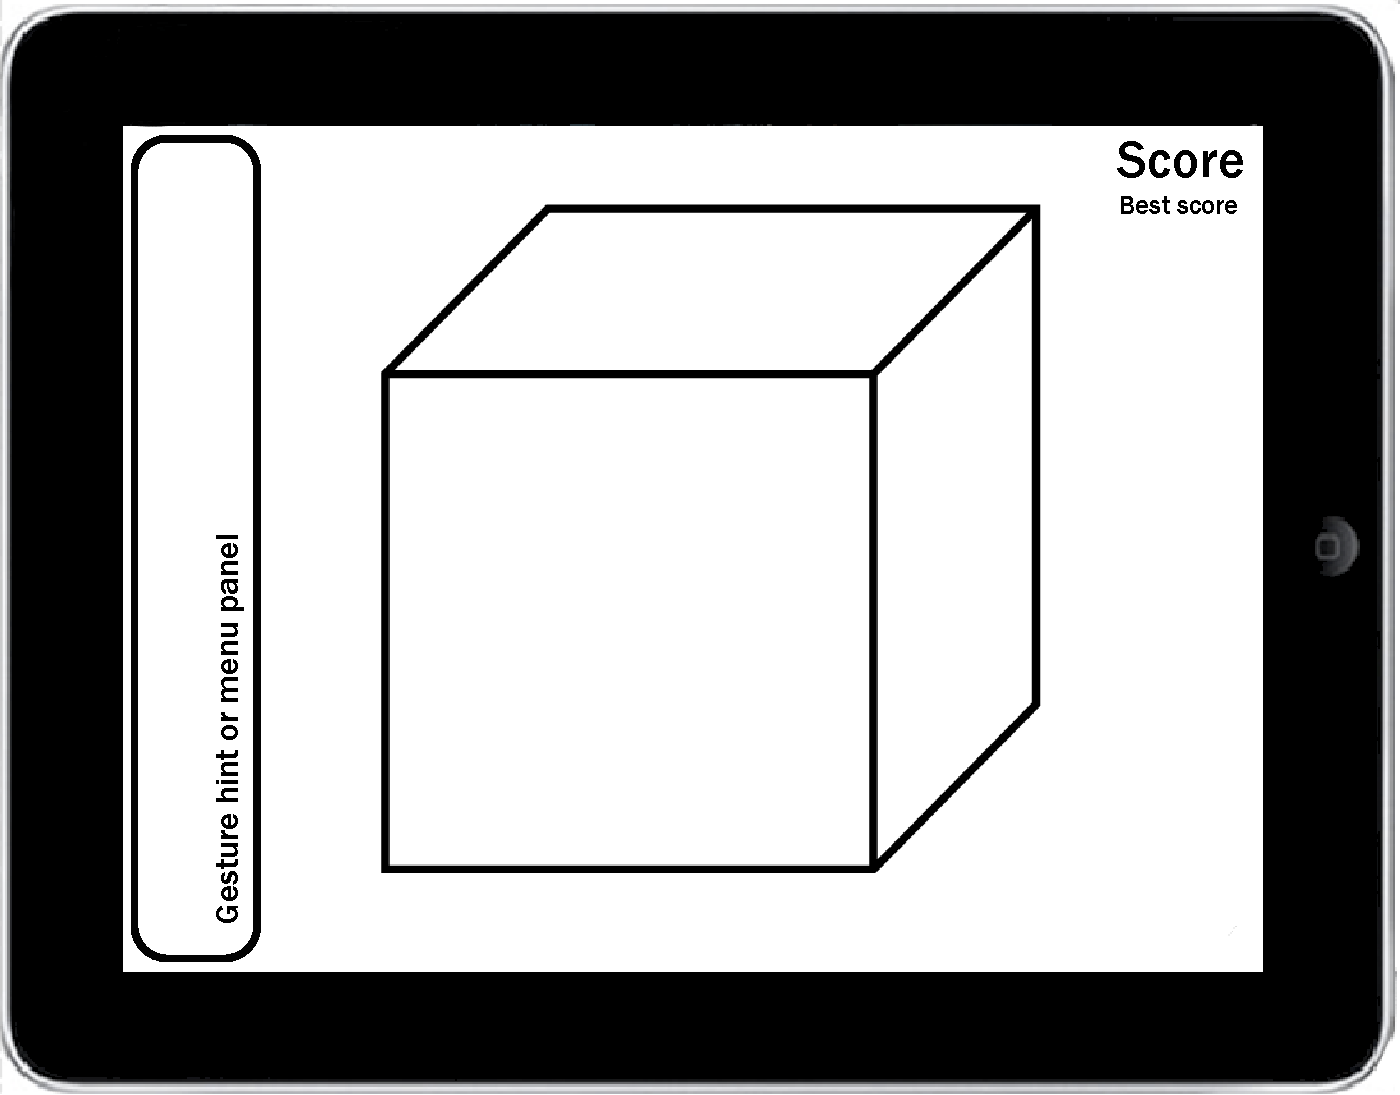
\includegraphics [scale=0.4]{interface.pdf}

  \end{center}
  \caption{An example of possible interface design.}
  \label{interface}
\end{figure}

A very simple, clean design will be used throughout \emph{Hexahedron}. That is, there will be minimal interface elements, as the majority of the move related commands will be executed by means of gestures or a single menu structure. This was chosen so that users are able to better focus on the core game-play without being distracted by extraneous elements. This is of importance as the purpose of the game is to elicit a flow state through game-play. In order to provide the three-dimensionality required by the game, shading will be used when colouring the cubes. In addition, a light-source will be positioned so that there is an illusion of depth. Finally, the overall \gls{shape} will also be rotated slightly so that the other faces are also slightly visible.

Four different colours will be used. These include red, blue, green and orange. Block movements will be accompanied by a brief animation which shows the movement of affected blocks before they reach their final positions.

A gesture hint panel will be provided on the left-hand side of the screen as initially there will be a large array of gestures to learn. This should provide a form of affordance to new players. Tapping one of the displayed icons on this bar will display the associated gesture and its meaning. In the direct manipulation version, this panel will serve as the block manipulation menu. This panel will also have the ability to be hidden. In order to hide the panel a three-finger swipe starting on the panel and ending at the edge of the screen will be used. Users will be able to redisplay the panel by using a three-finger swipe that starts at the edge of the screen and moves inwards. Apart from this, the only other interface elements visible will be the score, best previous score  and a \emph{New game} button (which will be placed on the left-hand menu). A basic mock-up of the described interface can be seen in Figure~\ref{interface}.

\subsection{Summary}
While \emph{Hexahedron} itself is fairly simple, its correspondence to a number of equally simple puzzle games, along with the addition of a third dimension should prove sufficiently compelling to induce a flow state. Furthermore, as gestures have been carefully selected to maximise the use of inherent affordances provided by their structure and relation to other gestures, this should serve to lessen the cognitive demands placed on the user. This is necessary as if users are unable to remember gestures they may feel as if they are not in control of the game~\citep{Wobb09}. This would, in turn, reduce the likelihood of achieving a flow state~\citep{Swee05}. Finally, due to the choice of movement controls, it should prove possible to implement both a direct manipulation and mixed interface version of the game without compromising the fundamental game-play and thus, gaming experience. Therefore this game should serve as an appropriate flow-inducing task in all three conditions. This allows the effect of interface type to be investigated within the context of touch-based gaming.

